\documentclass{article}
\usepackage[utf8]{inputenc}
\usepackage{titling}
\usepackage{graphicx}
\usepackage{xcolor}
\usepackage[colorlinks=true,linkcolor=darkgray, urlcolor =gray]{hyperref}
\usepackage[spanish]{babel}
\DeclareUnicodeCharacter{301}{~}
\usepackage{url}
\DeclareUnicodeCharacter{202F}{\,}


\title{Ejercicios Optativos 1}
\author{Cristina Díaz García}
\date{Diciembre 2018}

\renewcommand\maketitlehooka{\null\mbox{}\vfill}
\renewcommand\maketitlehookd{\vfill\null}


\begin{document}

\addcontentsline{toc}{section}{Índice general}

\begin{titlingpage}
\maketitle

\begin{center}

\includegraphics[scale=0.4]{images/comunicaciones.png} 
\end{center}

\end{titlingpage}

\newpage

\tableofcontents

\newpage

\section{I. Desarrollo de servicios no estándar}


\subsection{Ejercicio 1}.

1. Implementar un servicio de “eco” sobre UDP que lea las líneas de teclado hasta leer una
línea que contenga solamente un punto. Deberán tenerse en cuenta los siguientes requisitos de
implementación:
\begin{itemize}
\item El servidor UDP debe ser concurrente. Nota: tener en cuenta que no puedo tener dos
procesos UDP asociados al mismo puerto en una misma máquina.
\item Modelar el final del servicio con el envío de un “.” solo en una línea
(\textless{}CRLF\textgreater{}.\textless{}CRLF\textgreater{}).
\item El cliente UDP debe gestionar un temporizador de retransmisiones y establecer un
número máximo de retransmisiones.
\item Tanto el cliente como el servidor deben controlar que los mensajes del servicio de eco
pertenezcan todos a la misma transacción chequeando el puerto.
\end{itemize}



En este ejercicio se han implementado tres clases:

\begin{itemize}
\item \textbf{ClientUDP:} Es el cliente, al que se le pasan como argumentos al ejecutarlo, primero la dirección IP a la que conectarse, y segundo, el puerto. Si el puerto no se proporcionara, por defecto se usa el puerto 6789. Se introduce lo que se quiera, y al enviar, si el mensaje es un “.”, se cierra la conexión, y en caso contrario, se envía al servidor. Para cada envío, hay un tiempo máximo para recibir la respuesta (3 segundos), y un número máximo de intentos (7 intentos). Si no se recibiera respuesta, se cerraría la conexión.
\begin{center}
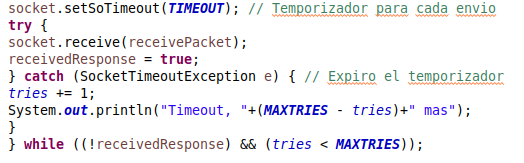
\includegraphics[scale=0.4]{images/UDPClient.png}
\end{center}
\item \textbf{ServerUDP: } Es el servidor, al que se le pasa como argumento el puerto por el que escuchar. La IP es localhost. Cada vez que un cliente se intenta conectar, se crea una instancia de \textit{ServerUDPImpl}, que es el que “gestiona” la conexión, es decir, es el que hace la función de eco.
\begin{center}
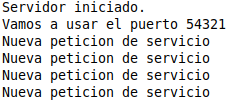
\includegraphics[scale=0.4]{images/UDPServer.png}
\end{center}
\item \textbf{ServerUDPImpl:} Recibe los mensajes del cliente y se los reenvía.
\end{itemize}

Las ventajas de la implementación con UDP es la rapidez de la conexión frente a la posible implementación en TCP. En esta implementación, uno de los problemas que tenemos es que estamos asumiendo que los argumentos se van a introducir tanto en el orden correcto como siendo los necesarios, es decir, no vamos a meter una IP incorrecta, ni vamos a introducir una palabra en vez de la IP correspondiente.

\section{II. Desarrollo de servicios estándar}

\subsection{Ejercicio 2}

2. Desarrollar un cliente de smtp simplificado que sea capaz únicamente de enviar mensajes
de correo electrónico. El protocolo SMTP está definido en el RFC 821 que se adjunta.
\begin{itemize}
\item Esta aplicación debe probarse en la máquina virtual de Linux, con el servidor de correo
estándar instalado en dicha máquina.
\item De los comandos del protocolo propuestos en el RFC sólo tendrán que implementar:
HELO, MAIL, RCPT, DATA, QUIT (implementación mínima, pág. 41).
\item La interfaz de usuario será muy sencilla:
\begin{itemize}
\item Compose
\begin{itemize}
\item Introducir una dirección de correo destino (opcionalmente podrían ser
varias)
\item Introducir el asunto del mensaje (el \textit{Subject})
\item Introducir el cuerpo del mensaje (podrá ser una o varias líneas, hasta
finalizar con un punto)
\end{itemize}
\item Quit
\begin{itemize}
\item Cerrar la conexión
\end{itemize}
\end{itemize}
\item Para comprobar que los mensajes enviados con tu aplicación han llegado
correctamente utiliza el cliente de correo estándar de Linux Mail. Un ejemplo sería:
\begin{center}
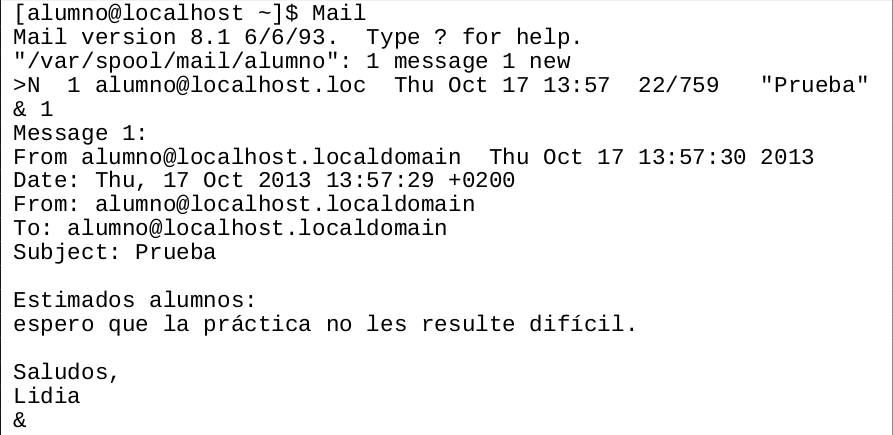
\includegraphics[scale=0.4]{images/ej.png}
\end{center}
\item \underline{Nota:} No usar la API javax.mail
\item \underline{Nota:} La dirección de correo de este usuario es nombre\_usuario\@nombre\_dominio. Para obtener el nombre del usuario actual, usar los siguientes métodos de Java:
\begin{itemize}
\item nombre\_usuario: System.getProperty(''user.name")
\item nombre\_dominio: InetAddress.getLocalHost().getHostName()
\end{itemize}
\end{itemize}

El cliente acepta la conexión en localhost y el puerto 25. Gestiona cuatro instrucciones básicas del protocolo SMTP para poder realizar el servicio: HELO, MAIL FROM:, RCPT TO: y DATA (que acaba cuando se introduce un punto). La información necesaria se introduce con un scanner por pantalla y comienza a enviar información.

\end{document}